\documentclass[]{politex}
% ========== Opções ==========
% pnumromarab - Numeração de páginas usando algarismos romanos na parte pré-textual e arábicos na parte textual
% abnttoc - Forçar paginação no sumário conforme ABNT (inclui "p." na frente das páginas)
% normalnum - Numeração contínua de figuras e tabelas
%	(caso contrário, a numeração é reiniciada a cada capítulo)
% draftprint - Ajusta as margens para impressão de rascunhos
%	(reduz a margem interna)
% twosideprint - Ajusta as margens para impressão frente e verso
% capsec - Forçar letras maiúsculas no título das seções
% espacosimples - Documento usando espaçamento simples
% espacoduplo - Documento usando espaçamento duplo
%	(o padrão é usar espaçamento 1.5)
% times - Tenta usar a fonte Times New Roman para o corpo do texto
% noindentfirst - Não indenta o primeiro parágrafo dos capítulos/seções


% ========== Packages ==========
\usepackage[utf8]{inputenc}
\usepackage{amsmath,amsthm,amsfonts,amssymb}
\usepackage{float}
\usepackage{graphicx,cite,enumerate}


% ========== Language options ==========
\usepackage[brazil]{babel}
%\usepackage[english]{babel}


% ========== ABNT (requer ABNTeX 2) ==========
%	http://www.ctan.org/tex-archive/macros/latex/contrib/abntex2
\usepackage[alf]{abntex2cite}

% Forçar o abntex2 a usar [ ] nas referências ao invés de ( )
%\citebrackets{[}{]}


% ========== Lorem ipsum ==========
\usepackage{blindtext}

% ========== PATH Relativo das Imagens ==========
\graphicspath{ {imagens/} }

% ========== Opções do documento ==========
% Título
\titulo{Sistema de Gerenciamento de Disciplinas de Projeto de Formatura do PCS}

% Autor
\autor{Lucas Arthur Felgueiras}

% Para múltiplos autores (TCC)
%\autor{Nome Sobrenome\\%
%		Nome Sobrenome\\%
%		Nome Sobrenome}

% Orientador / Coorientador
\orientador{Prof. Dr. Fabio Levy Siqueira}
% \coorientador{Nome do coorientador (opcional)}

% Tipo de documento
\tcc{de Computação}
%\dissertacao{Engenharia Elétrica}
%\teseDOC{Engenharia Elétrica}
%\teseLD
%\memorialLD

% Departamento e área de concentração
\departamento{Engenharia de Computação e Sistemas Digitais}
\areaConcentracao{Engenharia de Software}

% Local
\local{São Paulo}

% Ano
\data{2018}




\begin{document}
% ========== Capa e folhas de rosto ==========
\capa
\falsafolhaderosto
\folhaderosto


% ========== Folha de assinaturas (opcional) ==========
%\begin{folhadeaprovacao}
%	\assinatura{Prof.\ X}
%	\assinatura{Prof.\ Y}
%	\assinatura{Prof.\ Z}
%\end{folhadeaprovacao}


% ========== Ficha catalográfica ==========
% Fazer solicitação no site:
%	http://www.poli.usp.br/en/bibliotecas/servicos/catalogacao-na-publicacao.html


% ========== Dedicatória (opcional) ==========
\dedicatoria{Dedicatória}


% ========== Agradecimentos ==========
\begin{agradecimentos}

Thanks...

\end{agradecimentos}


% ========== Epígrafe (opcional) ==========
\epigrafe{%
	\emph{``Epígrafe''}
	\begin{flushright}
		-{}- Autor
	\end{flushright}
}


% ========== Resumo ==========
\begin{resumo}
Resumo...
%
\\[3\baselineskip]
%
\textbf{Palavras-Chave} -- Palavra, Palavra, Palavra, Palavra, Palavra.
\end{resumo}


% ========== Abstract ==========
\begin{abstract}
Abstract...
%
\\[3\baselineskip]
%
\textbf{Keywords} -- Word, Word, Word, Word, Word.
\end{abstract}


% ========== Listas (opcional) ==========
\listadefiguras
\listadetabelas

% ========== Listas definidas pelo usuário (opcional) ==========
\begin{pretextualsection}{Lista de símbolos}

Lista de símbolos...

\end{pretextualsection}

% ========== Sumário ==========
\sumario



% ========== Elementos textuais ==========

\part{Introdução}

\chapter{Motivação}

\section{Contexto}
Atualmente, o gerenciamento das duas disciplinas é realizado pelo Tidia-Ae, onde apenas os professores coordenadores da disciplina podem acessar o andamento da matéria, sem a participação dos demais envolvidos, em especial dos orientadores. Além disso, para compensar a ausência da participação no Tidia-Ae, os coordenadores precisam envolver os orientadores de maneira externa, para acompanhar o real \textit{status} do projeto, o que não é uma solução otimizada. Por fim, todo o processo de montagem de grupos, construção de bancas, parcerias para o evento e avaliações teóricas e práticas é realizada de maneira manual, o que gera um trabalho extenso para os coordenadores da disciplina.


\section{Problemas}
Além disso, não há um acompanhamento do status do projeto pelo Tidia-Ae, o que torna ele um simples repositório. O orientador acompanha o andamento do projeto apenas por intermédio do aluno, o que nem sempre gera uma abordagem eficiente, dado que ele depende do retorno do próprio aluno para saber atualizações, além de não ter uma central de fácil acesso para o orientador analisar os documentos relacionados.

Por fim, não há um sistema unificado que facilite os alunos que cursam a disciplina de consultar monografias anteriores de maneira estruturada e completamente on-line. O sistema visa, inicialmente, atacar essas demandas, de maneira a melhorar o andamento da disciplina como um todo. Futuramente, pode ser utilizada para outras disciplinas com estruturas semelhantes ao projeto de formatura.

\include{introducao/objetivo}
\chapter{Justificativa}

\section{Introdução}
Trabalhos relacionados aqui

\chapter{Organização do Trabalho}

\section{Introdução}
Este trabalho está organizado da seguinte forma:
\begin{itemize}
    \item
\end{itemize}


\part{Aspectos Conceituais}

\chapter{Levantamento de Requisitos}

\section{Introdução}
Em Engenharia de Software, é essencial o momento do levantamento de requisitos, dado que são eles que ditam o funcionamento do software a ser desenvolvido, alinha as expectativas dos \textit{stakeholders} e determinam os requisitos funcionais e não funcionais necessários para a aceitação. Neste projeto, não foi diferente: o primeiro processo de desenvolvimento foi o estudo de técnicas de levantamento de requisitos e uma série de entrevistas com os envolvidos no processo para gerar esses requisitos.

\section{Processo Genérico}

\subsection{\textit{Stakeholders}}

Para o levantamento de requisitos, foi usada uma das técnicas descritas em \cite{kurtbittnerianspence2002}, que consiste em levantar primeiramente os \textit{stakeholders} do projeto. Segundo \cite{kurtbittnerianspence2002}, a definição traduzida de \textit{stakeholder} é a seguinte:

\begin{citacaoLonga}
"Um indivíduo que é materialmente afetado pelo resultado do
sistema ou o(s) projeto(s) que produzem o sistema."
\end{citacaoLonga}

Ou seja, \textit{stakeholders} não são apenas os indivíduos que efetivamente usarão o sistema, mas sim todos os impactados sua existência. O livro divide os \textit{stakeholders} em 5 grupos:

\begin{itemize}
    \item Usuários: as pessoas que efetivamente usarão o sistema.
    \item Patrocinadores: os financiadores do projeto de software que gerará o sistema.
    \item Desenvolvedores: os responsáveis por desenvolver o sistema levantado pelo processo.
    \item Autoridades: órgãos reguladores que determinam regras para o uso de determinado software.
    \item Consumidores: empresas que compram esses softwares para serem usados.
\end{itemize}

\subsection{Entendimento dos Problemas}

Uma vez mapeado os \textit{stakeholders}, partimos para entender agora as dores que cada um possui e o que eles esperam com o produto final a ser desenvolvido. Alguns processos são sugeridos pelo livro\cite{kurtbittnerianspence2002}, como por exemplo:

\begin{itemize}
    \item Entrevistas: entrevistar os envolvidos e entender diretamente quais são suas dores e expectativas.
    \item Questionários: São úteis quando há um amplo número de \textit{stakeholders} envolvidos.
    \item Grupo Focal: Reunião com alguns representantes dos grupos de \textit{stakeholders} para entender e construir uma visão única sobre o projeto.
    \item Quadros de Aviso: É um tipo particular de grupo focal, onde o quadro serve como unificador da visão, com a diferença de não ter todos reunidos ao mesmo tempo.
    \item \textit{Workshops}: Eventos avisados com antecedência para entender melhor sobre o sistema, com a participação dos envolvidos.
    \item Revisões: Reuniões informais com o intuito de revisar documentos gerados com alguns envolvidos.
    \item Encenação: É uma técnica facilitadora usada em conjunto com \textit{workshops} para obter informações mais específicas ou \textit{feedbacks}.
\end{itemize}

Essencialmente, usando essas técnicas, devemos ser capazes de estabelecer relações do tipo problema-solução do sistema\cite{kurtbittnerianspence2002}:

\begin{itemize}
    \item O problema: a descrição do problema encontrado.
    \item Afeta: os \textit{stakeholders} afetados com o problema.
    \item O impacto: o que ele causa no dia-a-dia dos envolvidos.
    \item Uma solução boa: benefícios-chave da solução a ser proposta.
\end{itemize}


Com essa listagem de problemas levantados pelo processo de levantamento de requisitos, finalmente podemos partir para o levantamento real de requisitos, estabelecendo uma visão unificada do processo como um todo e como o software vai atuar no processo. Para isso, é saudável a elaboração de um documento unificando os pontos de vista dos \textit{stakeholders} e estabelecendo o que de fato será o sistema a ser desenvolvido. Esse documento é o Documento de Visão.

\subsection{Documento de Visão}

O documento de visão, segundo o livro\cite{kurtbittnerianspence2002}, traz a seguinte definição (traduzida):

\begin{citacaoLonga}
O Documento de Visão é o artefato do Rational Unified Process\cite{ibm2011} que capta todas as informações de requisitos. Como toda documentação de requisitos, seu objetivo principal é a comunicação.
\end{citacaoLonga}

Essencialmente, o Documento de Visão é o documento que reforça que todos os envolvidos estão alinhados sobre o que é o sistema, o que ele fará e como será seu processo-base de desenvolvimento, priorização e afins. O documento deve atender quatro funcionalidades básicas:

\begin{itemize}
    \item Base de alto nível (às vezes contratual) para os requisitos técnicos
    \item Processo de aprovação do projeto
    \item Maneiras de estabelecer o \textit{feedback} inicial
    \item Priorização e escopo do sistema
\end{itemize}

Existem diversos modelos de Documento de Visão, porém, em sua essência, atendem os seguintes tópicos\cite{kurtbittnerianspence2002}:

\begin{enumerate}
    \item Posicionamento: Como o sistema irá se posicionar no quesito de negócios? Há concorrentes que já resolvem o problema? Quais são seus diferenciais em relação a eles?
    \item \textit{Stakeholders} e usuários: Quem são os envolvidos direta e indiretamente com o desenvolvimento e a existência do sistema?
    \item Necessidades chave: Quais são as demandas que realmente precisam estar nos planos do sistema para satisfazer os envolvidos?
    \item Visão geral do produto: O que é o produto de fato? Quais são suas dependências, capacidades e alternativas ao seu desenvolvimento?
    \item Funcionalidades: Quais são as funcionalidades em alto nível do sistema, para que elas resolvam as necessidades chave listadas anteriormente?
    \item Outros requisitos do produto: Quais são os outros requisitos do sistema que não foram capturados como funcionalidades?
\end{enumerate}

Com o documento de visão em mãos, resta especificar de fato as funcionalidades do sistema usando uma metodologia adequada. No decorrer do trabalho, serão discutidas duas metodologias: Histórias de Usuário e Casos de Uso.

\section{Processo para o Projeto}

\subsection{\textit{Stakeholders}}

No caso do projeto, foi usado como base alguns processos de levantamento de requisitos do livro\cite{kurtbittnerianspence2002}.
Primeiramente, foram estabelecidos grupos de \textit{stakeholders} envolvidos com o projeto:

\begin{itemize}
    \item Coordenador: Responsáveis por administrarem as disciplinas de TCC 1 e 2 para os cursos de Engenharia de Computação Semestrais e Quadrimestrais.
    \item Orientador: Responsável por construir com os alunos a monografia.
    \item Técnico de Operação: Responsável por administrar novas funcionalidades futuras do sistema.
    \item Técnico do Evento: Responsável por cuidar da parte de infraestrutura dos eventos a serem realizados.
    \item Alunos: Os cursantes das disciplinas de TCC 1 e 2.
    \item Avaliador Teórico: Avaliam os projetos realizados, durante a banca de defesa da monografia.
    \item Avaliador Prático: Avaliam os projetos realizados, durante a feira de projetos de formatura.
\end{itemize}

Após entender melhor os grupos existentes de envolvidos, foram realizadas entrevistas com alguns desses \textit{stakeholders}, dentre eles:

\begin{itemize}
    \item Coordenadores da Disciplina: Profs. João Batista e Paulo Cugnasca
    \item Técnico Responsável pela Organização da Feira: Nilton Araújo
    \item Orientador e Avaliador Teórico: Prof. Fábio Levy Siqueira
\end{itemize}

Para o processo em questão, é valido reforçar alguns pontos importantes:

\begin{itemize}
    \item São 2 professores coordenadores, 2 técnicos, cerca de 50 alunos por ano de TCC e cerca de 20 professores orientadores do departamento de PCS.
    \item O ciclo da disciplinas de TCC dura 1 ano, sendo metade do tempo de especificação e metade de implementação.
    \item Atualmente, há a plataforma Tidia-AE existente para administrar as disciplinas. Porém, ela serve apenas como repositório de arquivos, sem a participação direta dos orientadores e sem infraestrutura de automação e comunicação rápida entre os envolvidos.
    \item Além disso, há o site do departamento, onde ficam as monografias mais recentes, também como simples repositório de arquivos.
\end{itemize}

Com isso, foram realizadas entrevistas com as pessoas citadas acima, para entender melhor o processo. A partir dessas entrevisas, diagramas de Modelo e Notação de Processos de Negócio (ou Business Process Model and Notation - BPMN) foram modelados para compreender o processo atual e, a partir dele, levantar os problemas-soluções do software, estabelecer o documento de visão e elaborar os casos de uso. Os diagramas BPMN estão na seção de apêndices do trabalho.

\subsection{Entendimento dos Problemas e Documento de Visão}

Após a geração do processo, os diagramas foram revistos com os coordenadores, para entender melhor o funcionamento e levantar os problemas encontrados. E, com base nesses problemas, o documento de visão foi gerado. A cópia da última versão está como apêndice deste trabalho.

Por fim, com a geração do documento de visão, foi possível seguir para a próxima etapa de especificação mais detalhada do sistema a ser desenvolvido, que será discutida nos capítulos a seguir.


\chapter{Histórias de Usuário}

\section{Introdução}
Para realizar as iterações de desenvolvimento, serão escritos, priorizados e detalhados diversos casos de uso responsáveis por delimitar o comportamento do sistema.

\section{Justificativa}
Como primeira abordagem a ser estudada para uso, escolhemos o Desenvolvimento Dirigido por Comportamento, que é uma técnica de desenvolvimento ágil que foca mais nas regras de negócio do que em detalhes técnicos em si. A princípio, seria desenvolver testes onde sua escrita seria em um nível maior do que se comparado com o Desenvolvimento Orientado a Testes.

Porém, um problema encontrado ao usar a abordagem citada acima seria a convergência natural ao uso de histórias de usuário, sendo essencial a participação constante das partes interessadas, o que pode dificultar o andamento do projeto. Sendo assim, descartamos seu uso, optando por linhas com a utilização de Casos de Uso.

\chapter{Casos de Uso}\label{chap:use-case-appendix}

\section{Introdução}

Neste apêndice consta os casos de uso escritos para o sistema em questão, usando o padrão explicado no capítulo de casos de uso\cite{funpar2001}.

\subsection{Cadastrar disciplinas}


\begin{enumerate}
    \item Breve Descrição


Coordenadores cadastram a disciplina, os alunos participantes e as atividades.


    \item Fluxo de Eventos

\begin{enumerate}
    \item Fluxo Básico

\begin{itemize}
    \item Coordenador insere disciplina, com os seguintes dados:

\begin{itemize}
    \item Modalidade (Sem/Quad)

    \item Data de início e data de término


\end{itemize}
    \item Coordenador importa planilha com alunos participantes, com os seguintes dados dos alunos

\begin{itemize}
    \item Nome

    \item E-mail

    \item Nº USP


\end{itemize}
    \item Coordenador insere uma nova atividade da disciplina, com os seguintes dados

\begin{itemize}
    \item Nome

    \item Data de entrega e arquivos relacionados

    \item Peso da atividade


\end{itemize}
    \item Sistema salva alunos novos, dispara e-mail ao aluno com seu acesso (login e senha) e vincula os existentes à disciplina e salva a disciplina
\end{itemize}

    \item Fluxos Alternativos

\begin{enumerate}
    \item Data de início é posterior a de término

\begin{enumerate}
    \item Sistema exibe novamente tela de cadastro da disciplina, alertando sobre erro


\end{enumerate}
    \item E-mail é inválido

\begin{enumerate}
    \item Sistema exibe novamente tela de cadastro da disciplina, alertando sobre erro


\end{enumerate}
    \item E-mail retornou

\begin{enumerate}
    \item Sistema envia e-mail ao coordenador com o aluno problemático




\end{enumerate}
\end{enumerate}
\end{enumerate}
    \item Requisitos Especiais


Não há


    \item Pré-condição


Coordenador deve estar logado


    \item Pós-condição

    Não há
\end{enumerate}

\subsection{Editar disciplinas}


\begin{enumerate}
    \item Breve Descrição


Coordenadores editam disciplinas, cadastrando atividades, editando alunos etc.


    \item Fluxo de Eventos

\begin{enumerate}
    \item Fluxo Básico

\begin{itemize}
    \item Coordenador edita início e término da disciplina, alunos participantes, com novos alunos ou removendo os já participantes

    \item Coordenador insere uma nova atividade da disciplina, com os seguintes dados

\begin{itemize}
    \item Nome

    \item Data de entrega

    \item Arquivos relacionados

    \item Peso da atividade


\end{itemize}
    \item Sistema salva novas atividades e as mudanças da disciplina
\end{itemize}

    \item Fluxos Alternativos



\end{enumerate}
    \item Requisitos Especiais


Não há


    \item Pré-condição


Coordenador deve estar logado


    \item Pós-condição

    Não há
\end{enumerate}

\subsection{Cadastrar professores}


\begin{enumerate}
    \item Breve Descrição


Coordenadores cadastram professores do departamento que podem orientar/co-orientar.


    \item Fluxo de Eventos

\begin{enumerate}
    \item Fluxo Básico

\begin{itemize}
    \item Coordenador insere os dados do professor

\begin{itemize}
    \item Nome 

    \item Número USP

    \item E-mail


\end{itemize}
    \item Sistema salva o professor, disparando e-mail para o professor cadastrado
\end{itemize}


    \item Fluxos Alternativos



\end{enumerate}
    \item Requisitos Especiais


Não há


    \item Pré-condição


Coordenador deve estar logado


    \item Pós-condição

    Não há
\end{enumerate}




















\subsection{Cadastrar grupos de trabalhos}


\begin{enumerate}
    \item Breve Descrição


Coordenadores cadastram os grupos com os temas e os orientadores, com a confirmação da participação do orientador no grupo.


    \item Fluxo de Eventos

\begin{enumerate}
    \item Fluxo Básico

\begin{itemize}
    \item Coordenador insere os dados do grupo

\begin{itemize}
    \item Título

    \item Alunos

    \item Orientador

    \item Co-orientador


\end{itemize}
    \item Sistema salva grupo e envia e-mail para o orientador, co-orientador e alunos

    \item Orientador valida participação no grupo

    \item Co-orientador valida participação no grupo
\end{itemize}


    \item Fluxos Alternativos

\begin{enumerate}
    \item Grupo não tem orientador

\begin{enumerate}
    \item Sistema cadastra grupo, enviando e-mail para os alunos com o aviso de urgência na escolha do orientador


\end{enumerate}
    \item Grupo não tem aluno

\begin{enumerate}
    \item Sistema retorna para a tela de cadastro de grupo, avisando sobre o erro de ausência de alunos
\end{enumerate}
\end{enumerate}


    \item Requisitos Especiais


Não há


    \item Pré-condição


Coordenador deve estar logado, alunos, orientadores e co-orientadores cadastrados


    \item Pós-condição

    Grupo confirmado
\end{enumerate}
\end{enumerate}

\subsection{Login}


\begin{enumerate}
    \item Breve Descrição


Alunos, Orientadores, Co-orientadores e Coordenadores acessam sistema de maneira tradicional ou via Senha Única USP (para pertencentes à USP).


    \item Fluxo de Eventos

\begin{enumerate}
    \item Fluxo Básico

\begin{itemize}
    \item Sistema mostra campos de login e senha

    \item Usuário insere seu e-mail e sua senha

    \item Sistema valida e-mail e senha

    \item Usuário acessa sistema
\end{itemize}


    \item Fluxos Alternativos

\begin{enumerate}
    \item Usuário erra credenciais

\begin{enumerate}
    \item Sistema retorna para tela de acesso ao sistema, exibindo mensagem de erro

    \item Retorna normalmente à situação de mostrar campos de login e senha


\end{enumerate}
    \item Usuário realiza login pela Senha Única da USP

\begin{enumerate}
    \item Usuário seleciona $``$Acessar pela Senha Única USP$"$ 

    \item Usuário é redirecionado para os sistemas USP

    \item Retorna para a situação de acesso ao sistema
\end{enumerate}
\end{enumerate}


    \item Requisitos Especiais


Integração via Shibboleth com os Sistemas USP


    \item Pré-condição


Não há


    \item Pós-condição

    Usuário dentro do sistema
\end{enumerate}
\end{enumerate}


\subsection{Entregar atividade}


\begin{enumerate}
    \item Breve Descrição


Alunos submetem no Google Drive arquivos da atividade para a leitura do orientador, co-orientador e coordenadores. Orientador e co-orientador revisam e dão seu aval de aprovação com a documentação.


    \item Fluxo de Eventos

\begin{enumerate}
    \item Fluxo Básico

\begin{itemize}
    \item Aluno submete arquivos nos respectivos espaços de atividades, que são carregados no Google Drive e deixa comentários adicionais sobre a entrega

    \item Sistema salva a entrega com o status da entrega da atividade para $``$Não avaliada$"$ 

    \item Sistema envia e-mail para Orientador e Co-orientador avisando de submissão

    \item Orientador baixa documentos submetidos

    \item Orientador avalia a entrega, faz comentários aos alunos e comentários exclusivos à coordenação com notas

    \item Sistema salva entrega e dispara e-mail com o resultado da avaliação para os alunos
\end{itemize}


    \item Fluxos Alternativos

\begin{enumerate}
    \item Data de submissão expirou (1)

\begin{enumerate}
    \item Aluno não consegue interagir com atividade, encerrando fluxo


\end{enumerate}
    \item Co-orientador realiza fluxo de revisão, antes do Orientador (4)

\begin{enumerate}
    \item Passos 5 - 7 ocorrem normalmente, trocando Orientador por Co-orientador


\end{enumerate}
    \item Co-orientador realiza fluxo de revisão, após Orientador (8)

\begin{enumerate}
    \item Sistema exibe detalhes da entrega, porém não permite edições do lado do Co-orientador, encerrando fluxo


\end{enumerate}
    \item Aluno submete nova entrega da atividade após ter feito uma submissão (1)

\begin{enumerate}
    \item Aluno vê status da avaliação

    \item Aluno realiza nova entrega da atividade, repetindo o caso de uso


\end{enumerate}
    \item Aluno submete entrega da atividade quando alguém do grupo já submeteu (1)

\begin{enumerate}
    \item Sistema exibe detalhes da entrega já realizada

    \item Aluno pode realizar nova entrega da atividade, passando por cima da entrega anterior e repetindo o caso de uso
\end{enumerate}
\end{enumerate}

    \item Requisitos Especiais


Não há


    \item Pré-condição


Atores devem estar autenticados e atividade deve estar cadastrada no sistema


    \item Pós-condição
    
    Não há
\end{enumerate}
\end{enumerate}


\subsection{Construir bancas práticas}


\begin{enumerate}
    \item Breve Descrição


Coordenadores selecionam os participantes da banca prática, já cadastrados no sistema, e os notifica com comentários sobre o evento.


    \item Fluxo de Eventos

\begin{enumerate}
    \item Fluxo Básico

\begin{itemize}
    \item Coordenador informa o dia da feira, a disciplina correspondente e as salas disponíveis para o evento, além de determinar o peso da avaliação da banca

    \item Sistema salva evento

    \item Coordenador seleciona evento recém criado.

    \item Sistema lista grupos do evento.

    \item Coordenador seleciona o grupo que deseja atribuir a sala e os convidados.

    \item Coordenador seleciona os convidados que avaliarão o grupo

    \item Sistema salva banca e envia e-mail para os convidados externos, avisando-os sobre sua participação

    \item Convidado acessa sistema e confirma participação na banca
\end{itemize}

    \item Fluxos Alternativos

Não há

\end{enumerate}
    \item Requisitos Especiais


Não há


    \item Pré-condição


Atores devem estar autenticados e grupo de trabalho deve estar cadastrado no sistema


    \item Pós-condição

    Não há
\end{enumerate}












\subsection{Construir bancas teóricas}


\begin{enumerate}
    \item Breve Descrição


Coordenadores escolhem participantes da banca teórica do grupo, selecionam o presidente da banca, realizam o agendamento do horário, validando inconsistências (participante já possui horário ocupado) e notificam os participantes por e-mail.


    \item Fluxo de Eventos

\begin{enumerate}
    \item Fluxo Básico

\begin{itemize}
    \item Coordenador informa o dia da banca, a disciplina correspondente e as salas disponíveis para o evento

    \item Sistema salva evento

    \item Coordenador seleciona evento recém criado.

    \item Sistema lista grupos do evento.

    \item Coordenador seleciona o grupo que deseja atribuir a sala e os convidados.

    \item Coordenador seleciona os avaliadores da banca e o horário da avaliação. O orientador é um dos pré-selecionados por padrão
\end{itemize}

    \item Fluxos Alternativos

\begin{enumerate}
    \item Convidado externo já possui banca nesse dia e horário

\begin{enumerate}
    \item Sistema barra criação de banca, alertando sobre qual convidado já possui agenda ocupada


\end{enumerate}
    \item Sala está ocupada no horário selecionado

\begin{enumerate}
    \item Sistema barra criação de banca, alertando sobre qual sala já possui agenda ocupada
\end{enumerate}
\end{enumerate}

 \item Requisitos Especiais


Não há


    \item Pré-condição


Atores devem estar autenticados e grupo de trabalho deve estar cadastrado no sistema


    \item Pós-condição

    Não há
\end{enumerate}
\end{enumerate}


\subsection{Listar entregas}


\begin{enumerate}
    \item Breve Descrição


Técnicos recebem os arquivos de impressão, com normalização do título, separados por grupo.


    \item Fluxo de Eventos

\begin{enumerate}
    \item Fluxo Básico

\begin{itemize}
    \item Coordenador lista todas as entregas finais de impressão (\textit{banner} e \textit{press-release})

    \item Sistema salva as listas de arquivos finais, com o nome normalizado e envia por e-mail para o técnico responsável
\end{itemize}

    \item Fluxos Alternativos

\begin{enumerate}
    \item Grupo de trabalho está com arquivo faltante

\begin{enumerate}
    \item Sistema envia e-mail para o grupo com entrega faltante, avisando para regularizar a situação com urgência.
\end{enumerate}
\end{enumerate}

    \item Requisitos Especiais


Não há


    \item Pré-condição


Atores devem estar autenticados e grupo de trabalho deve estar cadastrado no sistema


    \item Pós-condição

    Não há
\end{enumerate}
\end{enumerate}

\subsection{Listar necessidades adicionais}


\begin{enumerate}
    \item Breve Descrição


Técnicos recebem necessidades adicionais revisadas pelos orientadores, separadas por grupo.


    \item Fluxo de Eventos

\begin{enumerate}
    \item Fluxo Básico

\begin{itemize}
    \item Coordenador lista todos os comentários das entregas finais

    \item Sistema salva a lista de comentários e a envia por e-mail para o técnico responsável
\end{itemize}

    \item Fluxos Alternativos



\end{enumerate}
    \item Requisitos Especiais


Não há


    \item Pré-condição


Atores devem estar autenticados e grupo de trabalho deve estar cadastrado no sistema


    \item Pós-condição

    Não há
\end{enumerate}






















\subsection{Avaliar projetos práticos}


\begin{enumerate}
    \item Breve Descrição


Participantes da banca prática avaliam os projetos que estão envolvidos, limitando avaliações até o final do dia.


    \item Fluxo de Eventos

\begin{enumerate}
    \item Fluxo Básico

\begin{itemize}
    \item Convidado externo acessa espaço da banca, com detalhes do grupo e as entregas finais

    \item Convidado preenche os comentários e as notas de acordo com cada critério estabelecido para avaliação de bancas práticas

    \item Convidado salva avaliação
\end{itemize}

    \item Fluxos Alternativos

\begin{enumerate}
    \item Convidado tenta submeter avaliação em dia diferente ao da banca prática

\begin{enumerate}
    \item Avaliação é barrada, avisando o convidado de que a avaliação só pode ser feita exclusivamente no dia



\end{enumerate}
\end{enumerate}
\end{enumerate}
    \item Requisitos Especiais


Não há


    \item Pré-condição


Atores devem estar autenticados e grupo de trabalho deve estar cadastrado no sistema


    \item Pós-condição

    Não há
\end{enumerate}
















\subsection{Avaliar monografias teóricas}


\begin{enumerate}
    \item Breve Descrição


Participantes da banca teórica avaliam as monografias que estão envolvidas, gerando comentários e definindo o status do trabalho (aprovado, aprovado com correções, recuperação e reprovado), limitando avaliações até o final do dia.


    \item Fluxo de Eventos

\begin{enumerate}
    \item Fluxo Básico

\begin{itemize}
    \item Participante da banca acessa espaço da banca, com detalhes do grupo e as entregas parciais e finais.

    \item Participante preenche os comentários e as notas de acordo com cada critério estabelecido para avaliação de bancas teóricas

    \item Participante salva avaliação, com seu parecer para aprovação da monografia

    \item Presidente da banca vê avaliações dos outros envolvidos e determina o parecer final para a banca, com comentários para o grupo
\end{itemize}

    \item Fluxos Alternativos

Não há



\end{enumerate}
    \item Requisitos Especiais


Não há


    \item Pré-condição


Atores devem estar autenticados e grupo de trabalho deve estar cadastrado no sistema


    \item Pós-condição

    Não há
\end{enumerate}


\subsection{Calcular nota final dos projetos}


\begin{enumerate}
    \item Breve Descrição


Coordenadores determinam a fórmula para calcular as notas finais, com base nas entregas parciais durante as duas disciplinas e o sistema calcula as notas finais de todos os grupos participantes.


    \item Fluxo de Eventos

\begin{enumerate}
    \item Fluxo Básico

\begin{itemize}
    \item Coordenador escolhe as duas disciplinas (TCC1 e TCC2), a banca teórica e a feira prática que deseja obter as entregas

    \item Sistema salva fórmula de avaliação

    \item Sistema lista todos os grupos, com as notas calculadas e os estados de avaliação de cada grupo
\end{itemize}

    \item Fluxos Alternativos

\begin{enumerate}
    \item Coordenador não preenche algum dos campos necessários

\begin{enumerate}
    \item Sistema barra criação de fórmula de avaliação, avisando os campos faltantes


\end{enumerate}
    \item Grupo tem alguma avaliação faltante

\begin{enumerate}
    \item Sistema exibe grupo, mas com campo de Não Avaliado


\end{enumerate}
    \item Grupo vai para recuperação na avaliação da banca teórica

\begin{enumerate}
    \item A nota calculada é a nota da banca teórica, passando todas as outras avaliações realizadas ao longo das disciplinas


\end{enumerate}
    \item Grupo é reprovado na avaliação da banca teórica

\begin{enumerate}
    \item A nota calculada é a nota da banca teórica, passando todas as outras avaliações realizadas ao longo das disciplinas

Não há



\end{enumerate}
\end{enumerate}
\end{enumerate}
    \item Requisitos Especiais


Não há


    \item Pré-condição


Atores devem estar autenticados e grupo de trabalho deve estar cadastrado no sistema


    \item Pós-condição

    Não há
\end{enumerate}
\chapter{Testes}

\section{Introdução}
Para realizar as iterações de desenvolvimento, serão escritos, priorizados e detalhados diversos casos de uso responsáveis por delimitar o comportamento do sistema.

\section{Justificativa}
Como primeira abordagem a ser estudada para uso, escolhemos o Desenvolvimento Dirigido por Comportamento, que é uma técnica de desenvolvimento ágil que foca mais nas regras de negócio do que em detalhes técnicos em si. A princípio, seria desenvolver testes onde sua escrita seria em um nível maior do que se comparado com o Desenvolvimento Orientado a Testes.

Porém, um problema encontrado ao usar a abordagem citada acima seria a convergência natural ao uso de histórias de usuário, sendo essencial a participação constante das partes interessadas, o que pode dificultar o andamento do projeto. Sendo assim, descartamos seu uso, optando por linhas com a utilização de Casos de Uso.

\chapter{Validações}

\section{Introdução}
Para realizar as iterações de desenvolvimento, serão escritos, priorizados e detalhados diversos casos de uso responsáveis por delimitar o comportamento do sistema.

\section{Justificativa}
Como primeira abordagem a ser estudada para uso, escolhemos o Desenvolvimento Dirigido por Comportamento, que é uma técnica de desenvolvimento ágil que foca mais nas regras de negócio do que em detalhes técnicos em si. A princípio, seria desenvolver testes onde sua escrita seria em um nível maior do que se comparado com o Desenvolvimento Orientado a Testes.

Porém, um problema encontrado ao usar a abordagem citada acima seria a convergência natural ao uso de histórias de usuário, sendo essencial a participação constante das partes interessadas, o que pode dificultar o andamento do projeto. Sendo assim, descartamos seu uso, optando por linhas com a utilização de Casos de Uso.


\part{Tecnologias Utilizadas}

\chapter{\textit{Frameworks web}}

\section{Introdução}


\section{Django}

\chapter{Banco de Dados}

\section{Introdução}


\section{MariaDB}

\chapter{Ambientes de Teste}

\section{Introdução}


\section{Heroku}


\part{Metodologia de Trabalho}

\chapter{Processos de Levantamento de Requisitos}

\section{Introdução}


\chapter{Divisão em Iterações}

\section{Introdução}


\section{Django}


\part{Especificação de Requisitos do Sistema}

\chapter{Pontos Levantados nas Reuniões}

\section{Introdução}


\chapter{Requisitos Funcionais}

\section{Introdução}


\chapter{Requisitos Não Funcionais}

\section{Introdução}



\part{Projeto e Implementação}

\chapter{Elaboração da Estrutura do Sistema}

\section{Introdução}


\chapter{Problemas Iniciais de Implementação}

\section{Introdução}



\part{Teste e Validação}

\chapter{Validações}

\section{Introdução}


\chapter{Testes Executados}

\section{Introdução}


\chapter{Ambientes de Validação}

\section{Introdução}


\part{Considerações Finais}

\chapter{Resultados Alcançados}

\section{Introdução}


\chapter{Perspectivas}

\section{Introdução}




% ========== Referências ==========
% --- IEEE ---
%	http://www.ctan.org/tex-archive/macros/latex/contrib/IEEEtran
%\bibliographystyle{IEEEbib}

% --- ABNT (requer ABNTeX 2) ---
%	http://www.ctan.org/tex-archive/macros/latex/contrib/abntex2
\bibliographystyle{abntex2-num}

\bibliography{refs}

% ========== Apêndices (opcional) ==========
\apendice
\chapter{Documento de Visão}

\section{Introdução}
\subsection{Finalidade e Visão Geral do Documento}

O documento tem como finalidade coletar informações e unificar os pontos de vista sobre o sistema de gerenciamento da disciplina de TCC, como as necessidades encontradas e as causas para tais necessidades.

\subsection{Referências}

O site do departamento, bem como o Tidia-AE serviram como referência auxiliar para entender melhor as soluções atuais.

\section{Posicionamento}
\subsection{Descrição do Problema}

\begin{table}[!htb]
    \centering
    \caption{Descrição básica do problema}
    \label{my-label}
    \resizebox{\textwidth}{!}{\begin{tabular}{|l|l|lll}
        \cline{1-2}
        O problema de         & alto tempo e esforço para gerenciar a disciplina de maneira manual    &  &  &  \\ \cline{1-2}
        afeta                 & orientadores, alunos e coordenadores da disciplina            &  &  &  \\ \cline{1-2}
        cujo impacto é        & demora e esforço para notas, dificuldade para integração entre envolvidos, problemas de demanda     &  &  &  \\ \cline{1-2}
        uma boa solução seria & automatizar o processo e integrar os orientadores no processo &  &  &  \\ \cline{1-2}
    \end{tabular}}
\end{table}

\subsection{Sentença de Posição do Produto}

\begin{table}[!htb]
    \centering
    \caption{Sentença básica de posição do produto}
    \label{my-label}
    \resizebox{\textwidth}{!}{\begin{tabular}{|l|l|lll}
        \cline{1-2}
        Para            & alunos, orientadores, coordenadores e técnicos                                                                  &  &  &  \\ \cline{1-2}
        Que             & cursam ou estão envolvidos diretamente                                                            &  &  &  \\ \cline{1-2}
        O sistema       & de gerenciamento dos TCC's                                                                                      &  &  &  \\ \cline{1-2}
        Que             & armazena os TCC's anteriores e gerencia o TCC atual, realizando avaliação e controlando entregas                                                             &  &  &  \\ \cline{1-2}
        Ao contrário do & processo semi-manual de gerenciamento da disciplina, do Tidia-AE e do Site institucional em Wordpress                                                             &  &  &  \\ \cline{1-2}
        O sistema       & permite um acompanhamento dos envolvidos, bem como serve de histórico para os trabalhos anteriores &  &  &  \\ \cline{1-2}
    \end{tabular}}
\end{table}


\section{Descrições dos Envolvidos e Usuários}
\subsection{Resumo dos envolvidos}

Há alguns usuários que não estão diretamente envolvidos com o sistema, mas podem ser beneficiados ou interferem no sistema a ser desenvolvido:

\begin{itemize}
    \item Infraestrutura: Irá aplicar restrições tecnológicas e de negócio dado o ambiente desenvolvido.
    \item Secretaria do Departamento: Nem todos os integrantes irão usar o sistema, mas serão beneficiados pela automação de alguns processos internos da disciplina, diminuindo a demanda recorrente sobre a equipe, vide o fato deles gerenciarem as entregas das avaliações durante o processo.
\end{itemize}

\subsection{Resumo dos usuários}

Há diversos usuários que serão diretamente beneficiados com o sistema. São eles:

\begin{itemize}
    \item Coordenador: Responsáveis por administrarem as disciplinas de TCC 1 e 2 para os cursos de Engenharia de Computação Semestrais e Quadrimestrais.
    \item Orientador: Responsável por construír com os alunos a monografia.
    \item Técnico de Operação: Responsável por administrar novas funcionalidades futuras do sistema.
    \item Técnico do Evento: Responsável por cuidar da parte de infraestrutura dos eventos a serem realizados.
    \item Alunos: Os cursantes das disciplinas de TCC 1 e 2.
    \item Avaliador Teórico: Avaliam os projetos realizados, durante a banca de defesa.
    \item Avaliador Prático: Avaliam os projetos realizados, durante a feira de projetos de formatura.
\end{itemize}

\subsection{Representantes dos usuários}

Foram escolhidos representantes dos perfis citados acima, de maneira a facilitar conversas durante a especificação do documento.

\begin{itemize}
    \item João Batista/Paulo Cugnasca: Coordenadores das duas disciplinas.
    \item Edson Gomi: Professor orientador
    \item Selma: Avaliadora Teórica
    \item Nilton: Técnico do Evento
    \item Michelet: Técnico de Operação
    \item Fábio Levy: Responsável pela infraestrutura de hospedagem.
    \item Bruno Albertini: Responsável pela infraestrutura de hospedagem.
    \item Ex-aluno: Processo do lado do aluno cursante da disciplina.
\end{itemize}

\subsection{Ambiente do usuário}

Para o processo em questão, podemos reforçar alguns pontos importantes:

\begin{itemize}
    \item São 2 professores coordenadores, 2 técnicos, cerca de 50 alunos por ano de TCC e cerca de 20 professores orientadores do departamento de PCS.
    \item O ciclo da disciplinas de TCC dura 1 ano, sendo metade do tempo de especificação e metade de implementação.
    \item Atualmente, há a plataforma Tidia-AE existente para administrar as disciplinas. Porém, ela serve apenas como repositório de arquivos, sem a participação direta dos orientadores e sem infraestrutura de automação e comunicação rápida entre os envolvidos.
    \item Além disso, há o site do departamento, onde ficam as monografias mais recentes, também como simples repositório de arquivos.
\end{itemize}

\subsection{Principais necessidades do usuário}

Diversas necessidades foram encontradas, sendo agrupadas, estudadas e propostas soluções para atendê-las. A lista das necessidades encontradas está a seguir:

\begin{table}[!htb]
  \centering
  \caption{Necessidades encontradas}
  \label{my-label}
  \resizebox{\textwidth}{!}{\begin{tabular}{|l|l|l|l|}
    \hline
    Necessidade                                                                         & Prior. & Sol.Atual         & Sol. Proposta                                                \\ \hline
    Orientador, coordenadores e alunos têm dificuldades em manter contato              & 1      & E-mail, reuniões  & Colocar os orientadores nas entregas                         \\ \hline
    Busca de monografias antigas é complexa.                                            & 2      & Site do PCS       & Criar repositório de monografias finalizadas                 \\ \hline
    O processo de gerenciar empresas participantes é extremamente manual.               & 7      & Conversas         & Integrar empresas às monografias a serem avaliadas           \\ \hline
    Avaliadores têm dificuldade em acessar monografias.                                 & 4      & E-mail            & Permitir monografia de fácil acesso no sistema               \\ \hline
    Avaliação dos projetos é de maneira manual.                                         & 5      & Papel             & Permitir avaliação pelo sistema, inclusive de maneira mobile \\ \hline
    Encontrar temas e alunos e propor temas é um processo manual.                       & 9      & E-mail, conversas & Permitir alunos e orientadores proporem temas no sistema     \\ \hline
    O gerenciamento de recursos pela parte do técnico é depende dos alunos solicitarem. & 8      & E-mail, pen drive & Automatizar as demandas para os técnicos providenciarem      \\ \hline
    O processo de montagem da banca de TCC é manual.                                    & 6      & E-mail, conversas & Permitir montagem de bancas pelo sistema                     \\ \hline
    Fechar as notas finais é um processo exaustivo e com curto prazo.                   & 3      & Papel             & Automatizar o cálculo das notas finais                       \\ \hline
  \end{tabular}}
\end{table}

\subsection{Alternativas e concorrência}
\begin{itemize}
    \item Tidia-AE: Entregas pontuais, com acesso apenas aos integrantes do grupo e aos coordenadores da disciplina. Os orientadores ficam de fora das entregas principais, cabendo aos alunos realizarem essa comunicação de maneira extra-oficial.
    \item Moodle: Plataforma aberta conhecida no mercado para gerenciamento de disciplinas em geral. Serve para construir grupos e até incluir orientadores, porém não é uma alternativa simples e não possui funcionalidades de busca avançada.
    \item Site PCS (Wordpress): Apenas resultado final, de maneira pública, sem integração dos envolvidos no projeto.
\end{itemize}

\section{Visão Geral do Produto}
\subsection{Perspectiva do Produto}
O produto tem como missão automatizar o processo já existente para a disciplina, pois muitas funcionalidades propostas são realizadas de maneira manual ou simplificada, o que demanda muito tempo e esforço dos coordenadores e orientadores, tornando o processo frágil. Além disso, depende da iniciativa de todos os envolvidos, pois todo o processo de comunicação orientador-aluno é feito de maneira isolada do processo coordenador-aluno e coordenador-orientador.

\subsection{Suposições e Dependências}
A principal dependência encontrada é que o serviço deve ser hospedado na infraestrutura interna da Universidade de São Paulo, o que afetará a maneira como o produto será desenvolvido.
  
\section{Recursos do Produto}
O produto a ser desenvolvido deve atender as necessidades descritas anteriormente, ou seja, possíveis conteúdos interessantes são:

\begin{itemize}
    \item Facilitar comunicação orientador/coordenadores, permitindo que eles vejam todas as entregas dos alunos e validem, quando necessário.
    \item Buscar, de maneira pública, as monografias antigas, usando filtros e busca textual.
    \item Incluir avaliadores da feira no sistema para acompanhar monografias correntes.
    \item Permitir avaliação tanto da banca como da feira (com as empresas), permitindo acesso prévio ao conteúdo e facilitando a avaliação (de preferência na plataforma mobile).
    \item Permitir que orientadores, alunos e empresas proponham temas e consigam combinar grupos para realizar as propostas.
    \item Permitir aos técnicos gerenciarem recursos necessários para as apresentações (imprimir apresentações sem necessidade do aluno entregar arquivos via pen drive, por exemplo)
    \item Permitir a montagem de bancas de TCC, convidando os envolvidos e facilitando o acesso ao resultado final do aluno.
\end{itemize}
  
\section{Outros requisitos do produto}
Como principais requisitos não-funcionais importantes, vale ressaltar:

\begin{itemize}
    \item Confiabilidade: O sistema deve permanecer funcional durante as avaliações finais do curso, pois são cruciais para o bom andamento da matéria.
    \item Segurança: Os acessos às monografias em andamento devem ser apenas aos envolvidos diretos do trabalho. Além disso, as empresas só podem acessar o resultado final não revisado, para fins de avaliação.
    \item Usabilidade: O sistema deve ser bem intuitivo e de aprendizagem fácil, pelo tempo curto dos envolvidos na feira e pela mobilidade envolvida (avaliações pelo celular, por exemplo).
\end{itemize}

\chapter{Diagramas BPMN}

\section{Introdução}

Os diagramas de Modelo e Notação de Processos de Negócio (Business Process Model and Notation - BPMN) servem para modelar um processo de negócio de maneira a unificar a visão sobre aquele processo e encontrar possíveis otimizações para o mesmo processo.

Para o trabalho em questão, foram usados os diagramas para levantar o processo antes do sistema e após o sistema, assim evidenciamos a presença dele e em que ele ajuda no processo da disciplina.

Para este projeto, foi usada a ferramenta Draw.io\cite{drawio}, para elaborar os diagramas BPMN dos processos citados. Apesar de não ser uma ferramenta específica para esse tipo de diagrama, é uma ferramenta de diagramação simples e que possui bibliotecas de diversos tipos de diagramas, inclusive os de BPMN.

\section{Processo antes do Sistema}

Os diagramas BPMN foram gerados com base nas entrevistas realizadas durante o processo de levantamento de requisitos. Os resultados estão a seguir:

\clearpage
\subsection{TCC 1}

\begin{figure}[H]
    \centering
    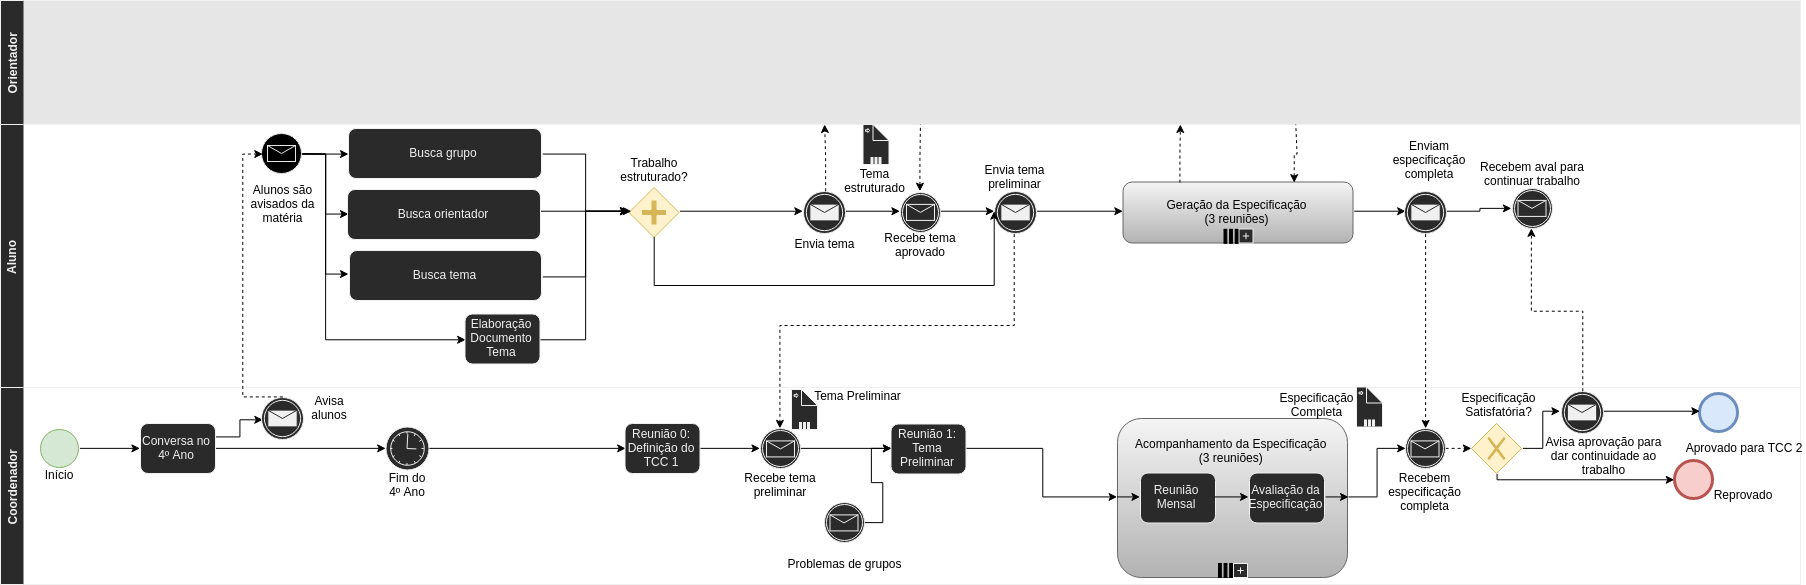
\includegraphics[angle=90, origin=c, scale=0.35]{bpmn-tcc1.png}
    \caption{Diagrama BPMN para a disciplina de TCC 1}
    \label{fig:bpmn-tcc1}
\end{figure}

\subsection{TCC 2}

\begin{figure}[H]
    \centering
    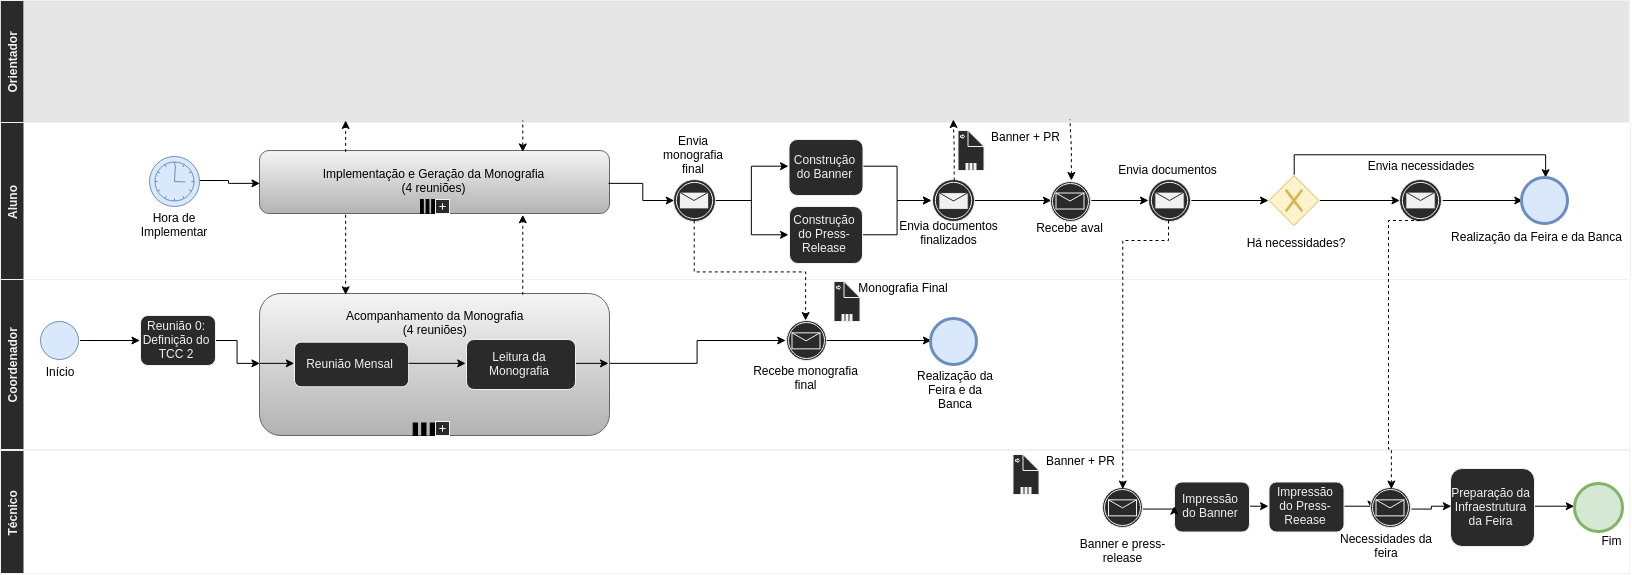
\includegraphics[angle=90, origin=c, scale=0.35]{bpmn-tcc2.png}
    \caption{Diagrama BPMN para a disciplina de TCC 2, antes dos eventos finais}
    \label{fig:bpmn-tcc2}
\end{figure}

\subsection{Banca e Feira}

\begin{figure}[H]
    \centering
    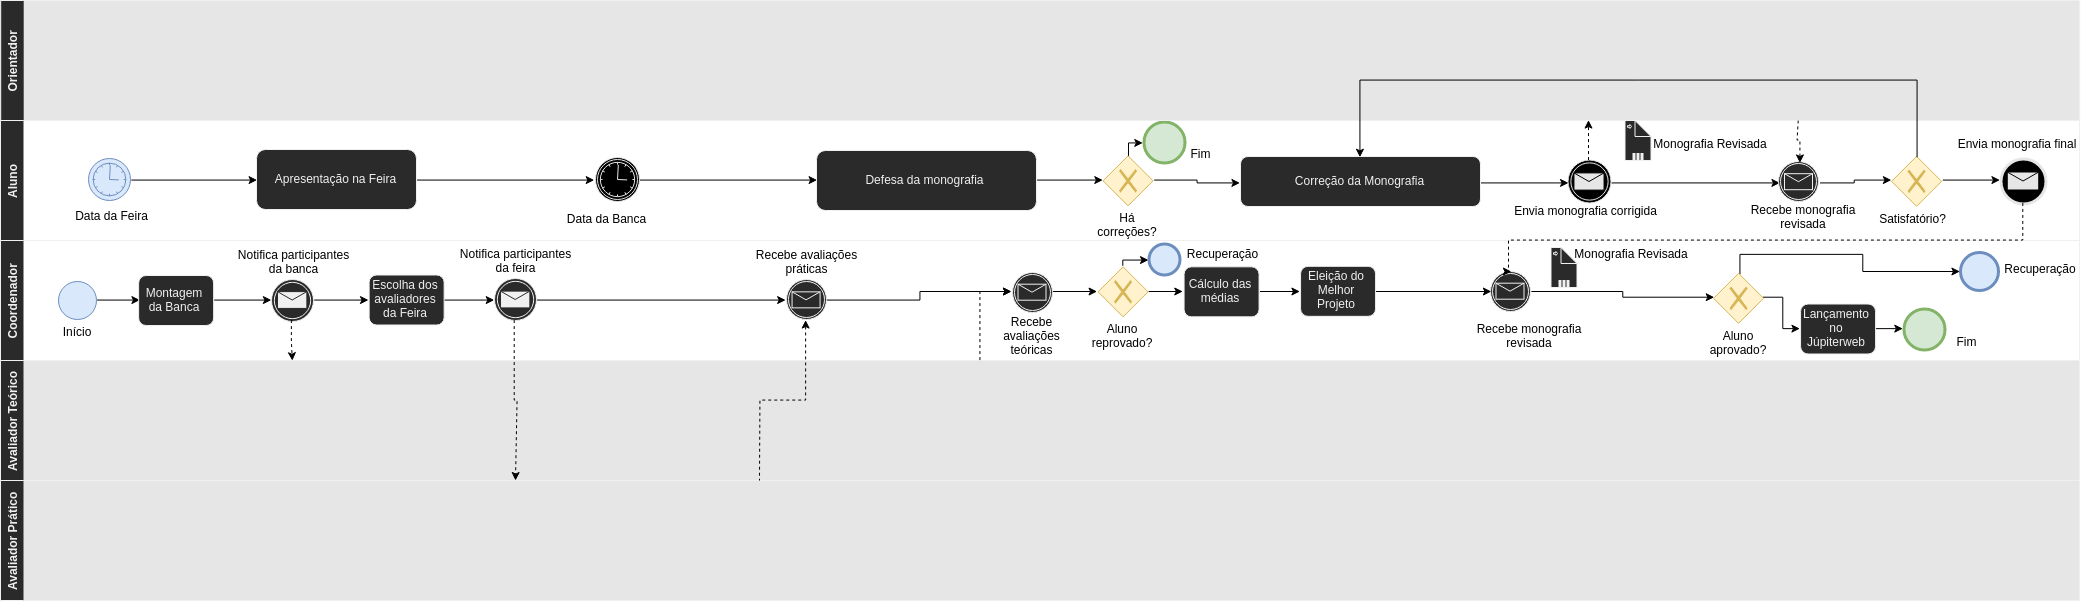
\includegraphics[angle=90, origin=c, scale=0.3]{bpmn-banca-feira.png}
    \caption{Diagrama BPMN para os eventos de banca e feira}
    \label{fig:bpmn-banca-feira}
\end{figure}

\subsection{Recuperação}

\begin{figure}[H]
    \centering
    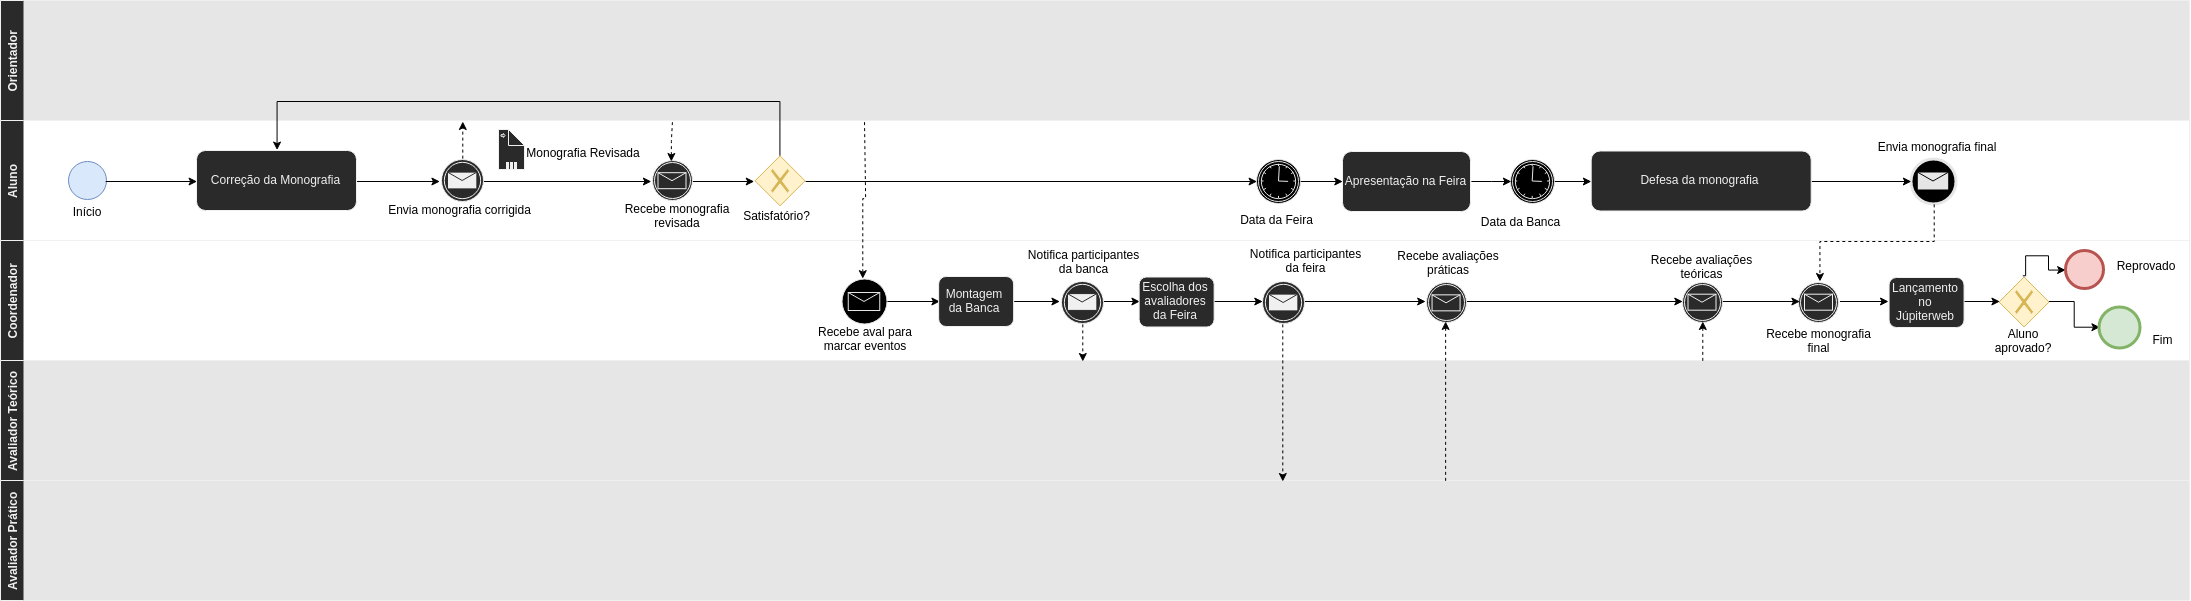
\includegraphics[angle=90, origin=c, scale=0.3]{bpmn-rec.png}
    \caption{Diagrama BPMN para a recuperação da disciplina de TCC 2}
    \label{fig:bpmn-rec}
\end{figure}

\section{Processo com o Sistema}

Já esses diagramas BPMN foram gerados com base no documento de visão, elaborado após o processo de levantamento de requisitos. Os resultados estão a seguir:

TO-DO




% ========== Anexos (opcional) ==========
\anexo

\end{document}
